\hyperref[sec:sec23]{\section{為什麼立法會議員變得越來越激進?}}
\label{sec:sec22}

因為香港立法會的議會和選舉制度都鼓勵議員變得激進。前文提到議會制度使得議員無法通過正常的議會手段,例如提出新建議或新政策來爭取表現,選民不能從議員或政黨提出和促使議案通過來辨認他們的政績。議員在立法會可做的,僅限於政府提出的議案在「執政聯盟」護航下通過前,提出一些質疑或不滿。而誰能在提出質疑或不滿時得到公眾的注意,就成為議員們爭取曝光的重要手段。立法會在提案和審議的先天缺陷,是某些議員走向激進的制度基礎。

理論上,如果議員的表現過於激進,脫離了社會主流期望,應該會在選舉中受到選民捨棄。換句話說,正常有效的選舉制度可為議員的激進化帶來一定制衡。不過,香港立法會的選舉制度十分不正常,地區直選的模式十分鼓勵議員的激進化。自特區成立以來,立法會的地區直選一直使用比例代表制當中的最大餘額法,而實踐起來則變成了世界各地普遍避免的多議席單票制。學界認為此制度選擇的原意是要打擊非建制陣營成立強大的政黨,而實際上也達到了此目的。不過它卻同時帶來另一個後果:立法會出現政黨碎片化和激進化,並反過來加深了政府的管治困難。

選舉方法和選舉結果有密切關係,同樣的民意在不同選舉方法下可產生極為不同的議會構成。一九九五年港英政府下最後一屆的立法局選舉中,地區直選採取單議席單票制當中的簡單多數制。由於在這制度下只要贏一票也算是贏,也就是所謂的「勝者全取」,假設一個派別在數個選區中每區各得三分之二選票,由於每區都取得多數選票,將可以全取100\%的議席。也說是說,這個制度會放大多數選民的支持,讓他們支持的派別得到較多的議席,學術上認為有利議會穩定。是次選舉中,香港就出現了歷史上唯一一次民主派議員佔多數的情況。

可以想像,特區政府不會容許同樣的選舉結果再次出現。結果政府決定在一九九八年把選舉制度改為比例代表制。理論上比例代表制可以帶來相對均衡的議席分佈。假設本來有五個各有一個議席的議區,可把它們合併為一個有五個議席的單一選區,候選人以名單方式參選並按得票的比例分配議席,例如拿到三分之二選票的名單則排首三位者為當選,拿到三分之一選票的名單則排首兩位者當選。表面上看,這應是一個相對公平的做法。

\begin{figure}[htbp]
    \centering
    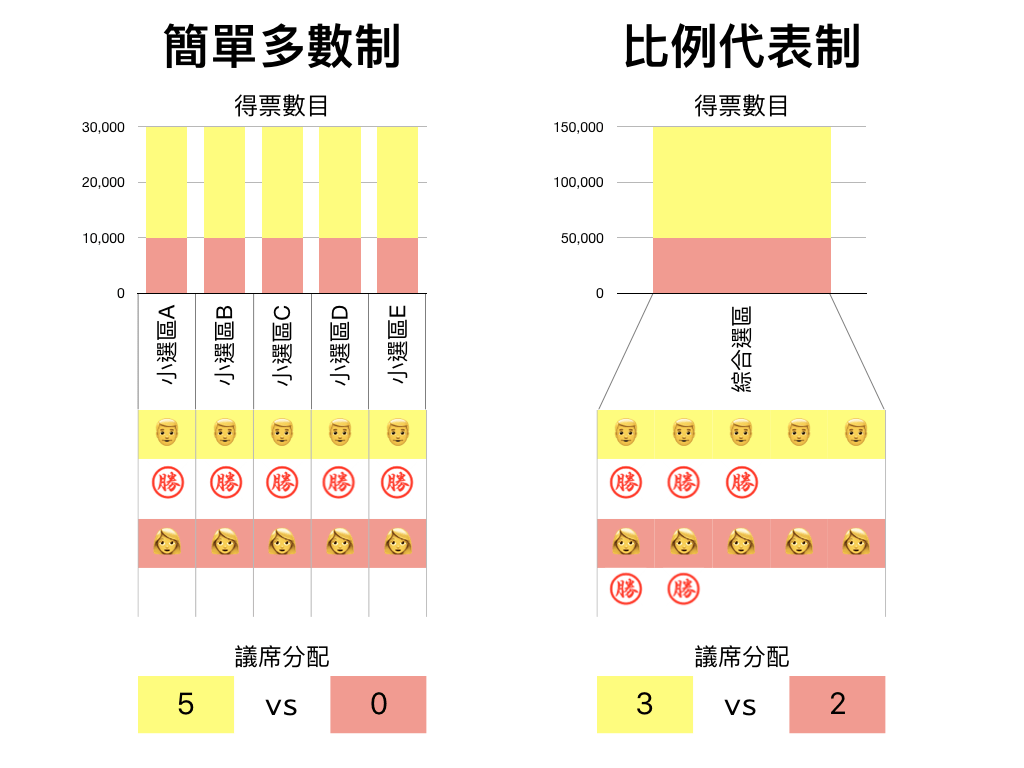
\includegraphics[width=0.7\textwidth]{c22/h-klesson1-035.png}
    \caption{同樣的選民選舉在不同的選舉制度下可帶來不同的結果} 
\end{figure}

不過在香港,考慮到整個議會本身不是由普選產生,功能界別的存在使得議席分佈本身已為建制陣營帶來優勢,如果在地區直選這一邊還要求一個相對公平的選舉方式,便會吊詭地反過來為議會帶來一個相對不公平的黨派構成。

選舉制度的更替明顯改變了立法會的政黨生態。民主派的最大政黨民主黨在一九九五年時於地區直選取得十二席,到了二零一六年時則跌到只得五席。加上功能界別的議席,一九九五年時民主黨的議員佔整個議會的32\%,到二零一六年時則跌到10\%,影響力大不如前。

打擊大政黨的後果,卻是製造政黨分裂和山頭林立的議會,為議會運作帶來混亂。細碎化的基礎在於最大餘額法使得任何追求多於一席的參選名單都等如浪費選票。舉個例,新界東和新界西選區分別有九個席位,即標準當選門檻為總票數的九分之一,或11\%,凡得此比例的名單均可穩奪一席。不過由於當沒有名單的票數多於標準門檻時,會直接把議席逐一分配與餘下得票順逐最高的名單,一般來說實際上只要7\%的選票已可穩奪一席。換言之,如果目標是一張名單取一席的話,候選人不用真的以爭取11\%的選票為目標,只要7\%左右已足夠。但如要同一張名單取兩席的話,就要11\%加7\%,即18\%的選票才能穩奪第二席。

這時候,任何排在名單第二名的候選人都會問:為什麼我要這麼笨排第二?如果我自己出來參選的話,當選的難度比排第二名要低得多了。這個制度設置,本質上鼓勵每一個政黨在選舉前要內部爭吵一次誰人排在名單首位,而每次爭輸了要排第二的都有極大誘因退黨獨立參選,試試能否靠一己之力當選。由於只要一百名當區選民聯署便可參選立法會,獨立參選在制度上的要求不高,政黨碎片化十分輕易就會出現。

從歷史去看,一九九八年的首屆立法會選舉中新界東有五席,共十一張名單參選。到了二零一六年的第五屆立法會選舉時,新界東有九席,共二十二張名單參選。名單數目之多,已使得連舉辦選舉論壇也變得十分困難,要找一個可以讓所有候選人一同出席的場地也不易,而每人可以發言的時間也變得十分有限。從結果去看,非建制陣營在二零一二年的第四屆立法會選舉中得二十七席,當中十九人來自有多於一名議員的政黨,其餘八人來為獨立議員或來自「一人政黨」(即只有一名立法會議員的政黨)。來到二零一六年,二十九名非建制陣營的議員當中,有十二人為獨立議員或來自「一人政黨」,見證了碎片化的趨勢。

\begin{figure}[htbp]
    \centering
    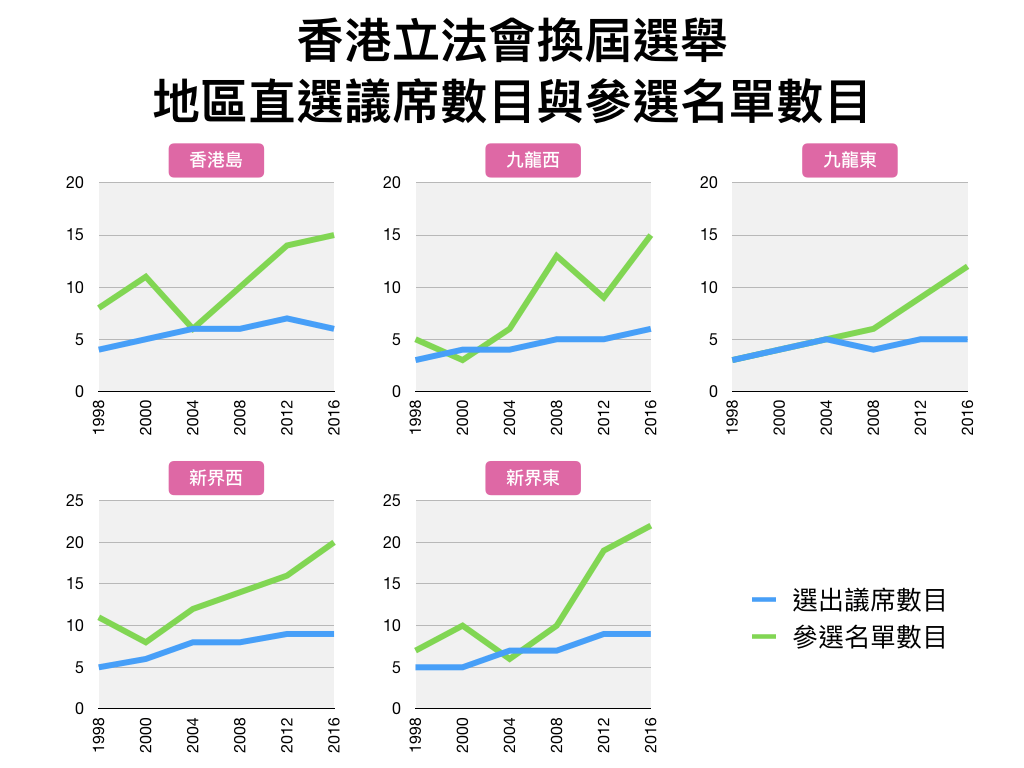
\includegraphics[width=0.7\textwidth]{c22/h-klesson1-036.png}
    \caption{立法會直選議席的參選名單數目近年快速增長} 
\end{figure}

順帶一提,較有規模的政黨為免處理名單排序的問題和嘗試爭取最多的議席,有時會主動分拆名單參選,即在同一個選區派出多於一張名單參選。如果不同名單之間的票數分配平均的話,這種做法可最大化選票的影響力。要做到這一點,就要組織支持者配票。台灣的政黨在這方面相對熟練,例如建議選民以出生月份或身份證號碼的最後一位數字來配票,達至平均分佈的效果。香港的選民並不慣於類似的配票方法,較為有效的方式往往是以「責任區」配票。以二零一六年立法會選舉為例,民建聯的陳克勤和葛珮帆同在新界東出選,其中陳克勤負責北區和大埔,葛珮帆負責沙田和西貢。結果陳克勤有78\%的選票來自北區和大埔,葛珮帆有88\%的選票來自沙田和西貢,策略十分成功。不過這種配票模式在非建制陣營卻並不成功,其中一個原因是非建制陣營的碎片化比建制陣營嚴重和明顯。

理論上,碎片化的問題會同樣衝擊建制陣營和非建制陣營。實際上,建制陣營在出選前都會接受協調,不服從者將會不能得到中央政府在港代理人的選舉資源支持。相對來說,非建制陣營本來就沒有太多選舉資源,也就失去團結一致的誘因。輿論往往會批評非建制陣營未能團結甚至互相攻擊,忽視了客觀上他們沒有很大誘因去團結,卻有不少誘因去分裂,黨派之爭只不過是其表徵而已。

剛才提到配票理論上可以把選票的影響力最大化,經歷數次港式比例代表制的選舉後,選民也發現配票的重要。當他們認為某候選人已有足夠支持度當選,又或其支持度已低得絕無可能當選時,就會考慮改為支持同一陣營而支持度處當選邊緣的候選人,試圖增加其選票的影響力。因此,臨近選舉時同陣營內「告急」和「棄保」的呼聲會十分熱烈,以左右選民的配票決定。然而由於民意調查的精密度有限,不可能支持嚴謹的配票行動,加上選民往往一窩蜂地按傳聞配票,以致每一屆都會出現「告急的候選人票數有餘,原來估計的票王卻意外落選」的情況。在二零一二年的換屆選舉當中,五區當中就有三區出現非建制陣營總得票較多,但因票數不均以致所得議席比建制陣營少的情況。

\begin{figure}[htbp]
    \centering
    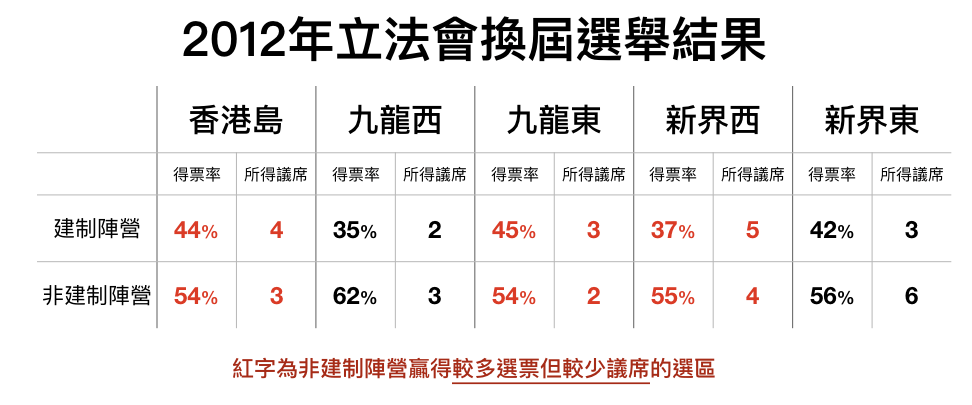
\includegraphics[width=0.7\textwidth]{c22/h-klesson1-037.png}
    \caption{配票失敗對非建制陣營的打擊十分嚴重} 
\end{figure}

簡而言之,港式比例代表制其實就是多議席單票制,每名選民只可投一票,而得票首若干名的候選人當選。正正因為多議席單票制會鼓勵「策略性投票」,不能反映選民的真正喜好,世界各國多已棄用。

回到激進化的問題,港式比例代表制是激進化的主要基礎。如果選舉以單議席單票制當中的簡單多數制實行,為免出現「鷸蚌相爭,漁人得利」的情況,不同派別都會有很大誘因協調出兩名候選人出來對決,而候選人的目標則是爭取選區內過半數投票者的支持。如是者,此制度下候選人的政綱往往會避免過於激進,以免得罪中間的游離選民。相反,在港式比例代表制當中,由於從政者只要討好大約二到三萬名選民便足以當選,即使會因而得罪另外數以十萬計的選民也不會影響其勝算,很自然就會有個別議員選擇走向激進,更能穩住他們的支持。

值得注意的,是立法會的碎片化本身就是中央政府想達到的目的。按曾於特區籌備委員會預備工作委員會負責政制工作的劉紹佳教授所術,當初設計立法會的選舉方式時的指導思想,正正包括確保行政主導和避免立法會出現單一大黨。前文提到,在一九九五年的最後一屆立法局選舉,民主黨以取得32\%的議席成為第一大黨;到了二零一六年的立法會選舉,民建聯只取得19\%的議席,已能成為第一大黨。選舉制度的改變促使民主黨失去第一大黨地位的同時,其他政黨也不能得到同等具影響力的位置。當立法會內的力量越見分散,立法會就不能成為香港政制內可以抗衡中央干預香港內部事務的力量。

關於立法會的碎片化,還有一個重要的註腳需要補充。理論上,即使選舉制度使得立法會黨派林立,理論上也不一定會導致混亂;畢竟議員可以在當選後合組聯盟,以獲得向政府施壓的力量,而這政治力量會反過來約束聯盟的參與者要顧及其他盟友,不能獨自行動。回到九八年特區首屆立法會選舉後,當時為了應對前所未見的金融危機,立法會內各派曾經不問政治立場共組「八黨聯盟」,在危機面前向市民顯示團結。由於他們在立法會有壓倒性的票數優勢,對政府的提案擁有否決權,所以提出的振興經濟和舒解民困方案都會獲得政府接納。不過,「八黨聯盟」在二零零四年後便未能繼續。據當時建制陣營的議員憶述,背後原因出於中聯辦的反對,認為強勢的立法會不符合原有「行政主導」的設想,所以要求建制陣營退出,轉為成為政府的「執政聯盟」。由是觀之,立法會出現亂象某程度上是中央政府樂意見到甚至積極推動而成的。

回到個別議員激進化的趨勢,不少民選議員近年選擇把議會當作是政治表演的場所,把街頭抗爭的手法帶進議事堂中,吸引傳媒的注意。他們的作為有時會被批評為不認真或不尊重議會莊嚴,個別議員就常常因被會議主席裁定違反議事規則而被逐離議事廳,因而被批評者譏為「提早下班」。但對於這些「反叛議員」的支持者來說,他們的議員在議事廳「搞事」就是履行選舉承諾,是一種「負責任」的表現。

隨著議會變成政治表演場所,議事廳的衝突也變得普遍,當中以二零一六年立法會宣誓就職案的影響特為深遠。《基本法》第一百零四條規定立法會議員在就職時「必須依法宣誓擁護中華人民共和國香港特別行政區基本法,效忠中華人民共和國香港特別行政區」,過往曾有立法會議員以各種方式於宣誓程序中表達不滿。例如梁國雄於二零零四年首次當選立法會議員後,就在宣讀誓詞前加上其他內容,又在宣讀以斷句方式干擾,立法會秘書處仍表示誓詞仍然有效。及後,不少議員都在宣誓前用道具或衣著表達政治立場,其中黃毓民在二零一二年時曾經一邊咳嗽一邊宣誓,也只被主席要求在下次大會重新宣誓。

來到二零一六年,部份獲選議員效法了這些先例,以各種方式在宣誓程序中表達政治立場。不過,這次他們的行動引發了廣泛的政治反響,結果當選人梁頌恆和游蕙禎未有被安排重新宣誓,政府隨即要求法庭禁止梁君彥再次為兩人監誓,全國人大常委則就《基本法》第一百零四條釋法,引起廣泛爭議。及後,政府再通過司法覆核取消本來已獲立法會確認宣誓有效的劉小麗、姚松炎、梁國雄和羅冠聰的議員資格,引發立法會獨立性和釋法追訴力的爭議。

說到底,議會變成政治表演場所只是問題表徵,後面是立法會本身出現制度失效,不能發揮正常議會的功能,因而改變了議員和選民對議會本身的期望。要解決問題,必須大幅改變立法會的制度本身。首先,立法會應全面取消功能界別,掃除一人多票和團體票的問題,重建立法會的認授,議員們才可以開展有實際意義的議政工作。至於選舉制度方面,學界和政界也有不少改革方案,例如實行比例代表制和單議席單票制並行的制度,把比例代表制的點票方式由最大餘額法改為最高均數法等方式,以及訂立最低當選門檻等,都可以減低碎片化的壓力。

就目前香港的政治形勢,無論是議會和選舉制度都難有理想的修改。因此,在立法會本來就難以發揮正常作用的前題下,立法會議事廳難免會變成政治表演的場所,畢竟最少有畫面可看,比乖乖坐下投贊成或反對票帶來更多的社會關注。議員的表現看起來好像不專重制度,但他們的行為剛剛好反映立法會的畸型制度。

\rule[-10pt]{15cm}{0.05em}

伸延閱讀:

馬嶽, 蔡子強(2003):《選舉制度的政治效果:港式比例代表制的經驗》,香港:香港城市大學出版社。

Cheung, CY. (2018). Stalemate in the Legislative Council of Hong Kong Disarticulation, fragmentation, and the political battleground of “One Country, Two Systems”, in Lui TL, Chiu SWK, and Yep R (eds) \textit{Routledge Handbook of Contemporary Hong Kong}, p132-155.